\chapter{METODE PENELITIAN}

Bab ini menjelaskan metode yang digunakan dalam penelitian secara sistematis, meliputi rancangan penelitian, sumber data, serta tahapan sistematis dalam pengembangan sistem. Penelitian ini merupakan dengan pendekatan rancang bangun sistem yang berfokus pada konstruksi \textit{Academic Knowledge Graph} yang diintegrasikan dengan  metode \textit{Hybrid Graph-based Retrieval-Augmented Generation} pada domain Informatika dan Komputer (Infokom).

\section{Dataset}

Penelitian ini memanfaatkan dataset yang dikembangkan secara mandiri karena belum terdapat dataset publik terintegrasi khusus untuk domain aktivitas akademik di Universitas Negeri Surabaya (UNESA). Dataset tersebut mencakup (1) profil peneliti (\cite{pddikti_db}), (2) publikasi dari \textit{Google Scholar} (\cite{google_scholar}), (3) riset internal UNESA (\cite{sinta_database}), serta (4) publikasi internasional yang terindeks di \textit{Scopus} (\cite{scopus_db}). Sumber-sumber ini dipilih guna membangun \textit{Academic Knowledge Graph} dengan tujuan memastikan bahwa dataset mencakup pengetahuan domain yang memadai untuk melakukan uji kueri.

Data difokuskan pada aktivitas akademik dosen di bidang kajian Informatika dan Komputer (Infokom) UNESA, mencakup enam program studi, Sains Data (14 dosen), Kecerdasan Artifisial (5 dosen), Teknik Informatika (9 dosen), Sistem Informasi (10 dosen), Magister Informatika (5 dosen), dan Teknik Elektro (13 dosen). Fokus ini bertujuan menghasilkan hubungan informasi yang relevan dan mendalam. Atribut dataset disesuaikan dengan kebutuhan sistem \textit{Question-Answering} terkait referensi akademik, dimulai dengan analisis kebutuhan data melalui \textit{competency questions} untuk memastikan fungsi dan ketepatan dataset. Struktur atribut dataset dapat dilihat pada Tabel~\ref{tab:deskripsi-dataset}.

\begin{longtable}{|P{0.15\linewidth}|P{0.22\linewidth}|P{0.13\linewidth}|P{0.4\linewidth}|}
    \caption{Struktur Atribut Dataset Penelitian} \label{tab:deskripsi-dataset} \\

    \hline
    \textbf{Dataset} & \textbf{Nama Atribut} & \textbf{Tipe Data} & \textbf{Deskripsi} \\ 
    \hline
    \endfirsthead
    
    \multicolumn{4}{c}{{\textit{ \ref{tab:deskripsi-dataset} (lanjutan).}}} \\
    \hline
    \textbf{Dataset} & \textbf{Nama Atribut} & \textbf{Tipe Data} & \textbf{Deskripsi} \\ 
    \hline
    \endhead
    
    \hline 
    \multicolumn{4}{r}{\textit{Bersambung ke halaman berikutnya}} \\
    \endfoot
    \hline
    \endlastfoot

    \textbf{Data Profil Dosen}
    & nidn / nip & String & Identitas unik dosen (NIDN atau NIP). \\ \hhline{|~|---|}
    & nama\_dosen & String & Nama lengkap dosen beserta gelar. \\ \hhline{|~|---|}
    & nama\_prodi & String & Program studi tempat dosen berafiliasi. \\ \hhline{|~|---|}
    & sinta\_id & String & ID dosen pada portal SINTA. \\ \hhline{|~|---|}
    & scholar\_id & String & ID profil dosen pada \textit{Google Scholar}. \\ \hhline{|~|---|}
    & scopus\_id & String & ID penulis dosen pada Scopus. \\ \hhline{|~|---|}
    & pendidikan & String & Jenjang pendidikan tertinggi dosen. \\ \hhline{|~|---|}
    & jabatan\_akademik & String & Jabatan fungsional akademik dosen. \\ 
    \hline

    \textbf{Data Scopus}
    & Title & String & Judul artikel yang terindeks Scopus. \\ \hhline{|~|---|}
    & Abstract & Text & Abstrak artikel untuk ekstraksi entitas dan relasi. \\ \hhline{|~|---|}
    & Authors & String & Daftar nama penulis artikel. \\ \hhline{|~|---|}
    & CiteScore\_2023 & Float & Nilai CiteScore jurnal tahun 2023. \\ \hhline{|~|---|}
    & Quartile & String & Kuartil kualitas jurnal (Q1--Q4). \\ \hhline{|~|---|}
    & Journal\_Source & String & Nama jurnal atau konferensi publikasi. \\ \hhline{|~|---|}
    & Link & String & URL atau DOI menuju halaman artikel. \\
    \hline

    \textbf{Data Riset Internal}
    & judul\_penelitian & String & Judul proyek penelitian yang didanai. \\ \hhline{|~|---|}
    & ketua\_peneliti & String & Nama dosen ketua peneliti. \\ \hhline{|~|---|}
    & sumber\_dana & String & Skema atau sumber pendanaan penelitian. \\ \hhline{|~|---|}
    & dana\_disetujui & Integer & Besaran dana penelitian yang disetujui (Rupiah). \\ 
    \hline

    \textbf{Data Scholar}
    & title & String & Judul publikasi pada \textit{Google Scholar}. \\ \hhline{|~|---|}
    & abstract & Text & Abstrak publikasi untuk ekstraksi entitas dan relasi. \\ \hhline{|~|---|}
    & authors & String & Daftar penulis publikasi. \\ \hhline{|~|---|}
    & citations & Integer & Jumlah sitasi publikasi. \\ \hhline{|~|---|}
    & year & Integer & Tahun terbit publikasi. \\ \hhline{|~|---|}
    & journal\_source & String & Nama jurnal, prosiding, atau media publikasi lain. \\ \hhline{|~|---|}
    & link & String & URL menuju halaman publikasi atau sumber asli. \\
\end{longtable}

\section{Alur Penelitian}

Alur penelitian ini dirancang sebagai rangkaian proses terstruktur untuk membangun \textit{Academic Knowledge Graph} dan mengimplementasikan \textit{Hybrid Graph-RAG} sebagai asisten pencarian literatur pada domain \textit{Informatika dan Komputer} di Universitas Negeri Surabaya (UNESA). Setiap tahapan pada \ref{fig:alur-penelitian} dijelaskan secara operasional, mulai dari pengumpulan data multi-sumber, pembersihan dan validasi kualitas data, penyatuan entitas lintas sumber, hingga ekstraksi informasi untuk membentuk graf dan indeks semantik yang digunakan pada tahap \textit{retrieval} dan \textit{generation}.

\begin{figure}[htbp]
    \centering
    \includegraphics[width=1.0\textwidth]{Gambar/alur penelitian.png}
    \caption{Diagram alur penelitian}
    \label{fig:alur-penelitian}
\end{figure}

\begin{enumerate}[label=\textbf{\arabic*.}, leftmargin=*, itemsep=10pt]

    % 1. Data Collection
    \item \textbf{\textit{Data Collection}}
    
    Tahap ini berfokus pada \textit{Ingestion} dataset akademik secara mandiri untuk domain Infokom UNESA. Data dikumpulkan dengan menyusun profil 56 dosen dari website PDDikti dan mengakuisisi identitas unik mereka (\textit{NIDN, SINTA ID, Scholar ID,} dan \textit{Scopus ID}) sebagai kunci integrasi lintas platform. Akuisisi data dilakukan melalui empat medium dibawah ini:
    
    \begin{itemize}[leftmargin=0.75cm, itemsep=5pt]  
        \item \textbf{Data Identitas (PDDikti \& SimCV):} Sumber utama identitas dosen diperoleh melalui \textit{web scraping} dari PDDikti \citep{pddikti_db} dan SimCV UNESA menggunakan \textit{Selenium}.  
        
        \item \textbf{Publikasi Umum (\textit{Google Scholar}):} Menyediakan konten ilmiah yang luas, data dikumpulkan melalui \textit{third-party scraping API} berdasarkan \textit{Scholar ID} \citep{google_scholar} dosen informatika dan komputer (infokom), menghasilkan sekitar 1.960 entri.  
        
        \item \textbf{Riset Institusional (SINTA):} Menggambarkan riwayat penelitian nasional dosen dari tahun 2013 hingga 2025, data diambil dari SINTA \citep{sinta_database} berdasarkan \textit{Scholar ID} \citep{google_scholar} dosen informatika dan komputer (infokom), mencakup judul penelitian, pendanaan, dan anggota, dengan total 440 entri.  
    
        \item \textbf{Publikasi Global (\textit{Scopus} via SciVal):} Melengkapi publikasi yang terindeks secara internasional, metadata diunduh dari situs SciVal \citep{scopus_db} dalam format \textit{CSV}, menghasilkan 2.537 entri publikasi mentah yang berafiliasi dengan UNESA dan akan disaring berdasarkan \textit{Subject Area}.  
    \end{itemize}
    
    % 2. Data Analysis and Cleaning
    \item \textbf{\textit{Data Cleansing}}
    
    \hspace*{0.75cm}Tahap ini merapikan dan menyeragamkan struktur data agar siap diproses pada tahap berikutnya. Pembersihan dilakukan pada level skema dan konten, meliputi penyamaan nama kolom lintas sumber seperti judul, penulis, tautan/DOI), serta Pada kolom teks (judul dan abstrak), dilakukan normalisasi dasar dan penghapusan entri tidak informatif. Abstrak yang kosong atau terlalu pendek, $<50$ kata dikeluarkan dari jalur ekstraksi karena tidak memadai untuk pembentukan representasi semantik dan ekstraksi entitas.

    % 3. Data Validation
    \item \textbf{\textit{Data Validation}}

    \hspace*{0.75cm}Setelah data dibersihkan, dilakukan validasi untuk memastikan konsistensi kualitas data sebelum diintegrasikan. Validasi mencakup pemeriksaan kelengkapan atribut kunci seperti NIDN untuk dosen dan DOI untuk publikasi, konsistensi tipe data, serta deteksi duplikasi baris pada masing-masing sumber. Pada data SciVal, juga dipastikan bahwa data yang dipertahankan benar-benar berada pada \textit{Subject Area} \textbf{Computer Science} sehingga domain Informatika dan Komputer tetap terjaga.

    \item \textbf{\textit{Entity Resolution}}  
    
    \hspace*{0.75cm}Tahap ini bertujuan menggabungkan rekaman dari berbagai sumber yang merujuk pada entitas dunia nyata yang sama untuk menghindari duplikasi simpul pada graf. Proses \textit{Entity Alignment} mengutamakan pencocokan kunci unik secara deterministik, dengan metode kemiripan teks sebagai pendukung jika atribut kunci tidak tersedia.  
        
    \begin{itemize}[leftmargin=0.75cm, itemsep=5pt]  
        \item \textbf{Resolusi Dosen:} Identitas dosen disatukan lintas sumber menggunakan NIDN sebagai kunci utama, memastikan variasi penulisan nama tetap merujuk pada satu entitas.  
        
        \item \textbf{Resolusi Publikasi:} Data publikasi dari \textit{Scopus} dan \textit{Google Scholar} digabungkan dengan DOI sebagai identitas unik. jika tidak ada DOI, pencocokan dilakukan berdasarkan kombinasi judul, tahun, dan penulis.  
        
        \item \textbf{Resolusi Riset:} Entri penelitian disatukan berdasarkan kesamaan judul, tahun, dan ketua peneliti, menjamin setiap proyek tercatat sebagai entitas tunggal meskipun dari laporan berbeda.  
    \end{itemize}

     % A. Construction of the Knowledge Graph
    \item \textbf{Konstruksi \textit{Knowledge Graph}}
    
    \hspace*{0.75cm}Tahap ini mengaktualisasikan komponen yang diistilahkan \textit{Index Flow} melalui sebuah \textit{information extraction pipeline} yang memproses dua jenis tipe data, yaitu data terstruktur (profil dosen, metadata riset, dan metadata publikasi) serta data tidak terstruktur (abstrak). Luaran tahap ini adalah (i) \textit{Academic Knowledge Graph} pada basis data graf Neo4j dan (ii) indeks semantik pada basis data vektor untuk mendukung \textit{retrieval}. Alur \textit{pipeline} mengikuti skema pada \ref{fig:kg-construction}.

    % Placeholder Gambar 2
    \begin{figure}[htbp]
        \centering
        \includegraphics[width=0.95\textwidth]{Gambar/construct kg.png}
        \caption{\textit{Index Flow} dan konstruksi graf pada \textit{Academic Graph-RAG}}
        \label{fig:kg-construction}
    \end{figure}
        
    \begin{enumerate}[label=\textbf{\arabic*.}, leftmargin=0.75cm, itemsep=5pt]
        \item \textbf{\textit{Text Processing}}
        
        \hspace*{0.75cm}Dokumen teks mentah (abstrak publikasi dan metadata penelitian) diproses terlebih dahulu. Karena model bahasa memiliki batasan panjang \textit{input}, diterapkan teknik \textit{text chunking} untuk memecah teks panjang menjadi segmen yang lebih kecil namun tetap utuh secara semantik. Selain itu, dilakukan pembersihan teks (\textit{text cleaning}) dan normalisasi karakter untuk meminimalkan \textit{noise} sebelum masuk ke proses inferensi model.
    
        \item \textbf{\textit{Coreference Resolution}}

        \hspace*{0.75cm}Tahap ini bertujuan memperjelas rujukan dalam teks dengan mengganti kata ganti dengan nama entitas asli. Menggunakan \textit{Neuralcoref} \citep{clark2016deepreinforcementlearningmentionranking}, model berbasis \textit{SpaCy} dan \textit{deep reinforcement learning}, tahap ini mengidentifikasi dan menghubungkan referensi antar entitas, menjadikan teks lebih koheren dan memudahkan ekstraksi relasi entitas selanjutnya.

        \item \textbf{\textit{Knowledge Extraction} (NER dan RE)}
        
        \hspace*{0.75cm}Ekstraksi dilakukan secara sinergis menggunakan dua model generalis, \textbf{GLiNER} \citep{zaratiana2023gliner} untuk mengidentifikasi entitas spesifik seperti \textit{Task, Method}, dan \textit{Metric}, serta \textbf{GliRel} \citep{boylan2025glirelgeneralistmodel} untuk memetakan hubungan (\textit{Relation Extraction}) antar entitas tersebut. Hasil dari tahap ini adalah \textit{Lexical Graph}, yaitu jaringan awal yang menangkap fakta-fakta mentah dalam bentuk \textit{triplet} pengetahuan

        \item \textbf{\textit{Entity Linking}}  
        
        \hspace*{0.75cm}Tahap ini memvalidasi dan menormalkan simpul dalam \textit{Lexical Graph} dengan \textit{Entity Linking} menggunakan \textit{Wikifier API} untuk menghubungkan entitas dari dokumen akademik ke konsep \textit{Wikipedia} yang relevan. Ini membantu menyatukan variasi penulisan seperti "DL", "Deep Learning", dan "pembelajaran mendalam" menjadi satu entitas unik dalam \textit{Knowledge Graph}. \textit{Wikifier} adalah layanan web yang otomatis menganotasi teks dengan entitas \textit{Wikipedia}, mendukung hingga 100 bahasa.
    
        \item \textbf{\textit{Indexing}}  
        
        \hspace*{0.75cm}Tahap terakhir adalah menyimpan hasil ekstraksi ke basis data dengan dua mekanisme paralel yang terhubung lewat referensi potongan teks (\textit{chunk reference}):  
        
        \begin{enumerate}[label=\textbf{\alph*.}, leftmargin=0.75cm, itemsep=5pt]  
            \item \textbf{\textit{Vector Indexing}}  
            
            \hspace*{0.75cm}Menyimpan teks abstrak agar dapat dicari berdasarkan makna, bukan hanya kata kunci, menggunakan \textit{Vector Store} (VS). Teks dipotong menjadi \textit{chunks} 2.024 karakter dengan overlap 50 karakter, lalu diubah menjadi vektor dengan model \texttt{all-MiniLM-L6-v2} dan disimpan di basis data vektor \textit{Weaviate} untuk pencarian cepat dan akurat.
            
            \item \textbf{\textit{Graph Indexing}}  
            
            \hspace*{0.75cm}\textit{Triplet} entitas dan relasi dimuat ke basis data graf \textit{Neo4j} untuk membentuk jaringan pengetahuan. Pemuatan dilakukan otomatis dengan \textit{Neo4j Python driver} atau \textit{Cypher queries} yang membuat node dan edge dari daftar entitas dan relasi hasil ekstraksi.  
            
            \end{enumerate}  
        \end{enumerate}
        
    % B. Academic Graph-RAG Modelling
    \item \textit{\textbf{AcademicRAG Modelling}}

    \hspace*{0.75cm}Tahap ini bertujuan untuk menjalankan proses pencarian informasi yang cerdas (Query Flow). Berbeda dengan pencarian biasa, sistem ini menggunakan struktur graf untuk memandu AI dalam menemukan jawaban yang paling relevan. Proses ini dibagi menjadi empat langkah utama seperti pada ~\ref{fig:downstream-task}
        
    \begin{figure}[htbp]
        \centering
        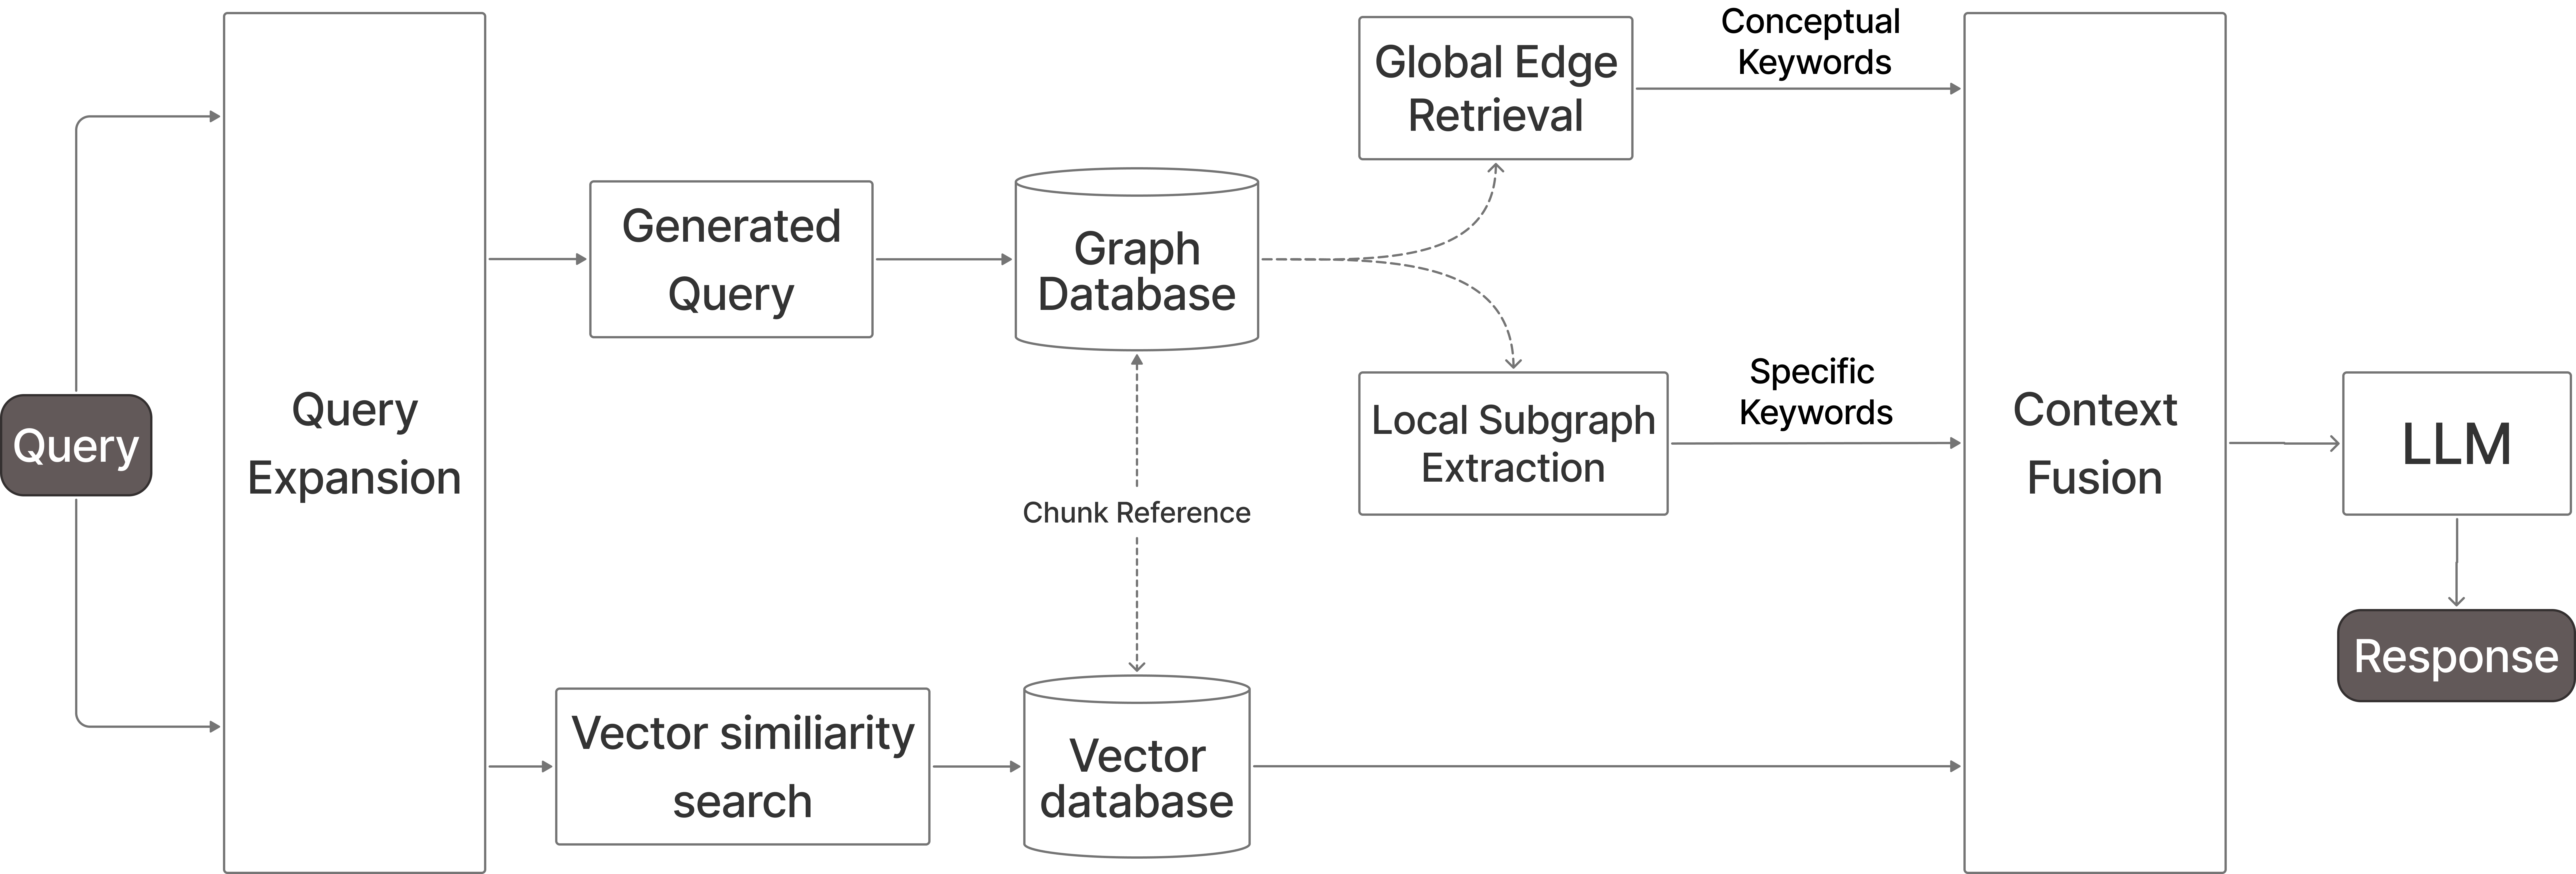
\includegraphics[width=1\textwidth]{Gambar/alur graph rag new.png}
        \caption{\textit{Query Flow} pada \textit{Academic Graph-RAG}}
        \label{fig:downstream-task}
    \end{figure}
    
    \begin{enumerate}[label=\textbf{\alph*.}, leftmargin=*, itemsep=5pt]
    
        \item \textbf{Pengambilan Kata Kunci Berbasis Petunjuk (\textit{Clues})}

        \hspace*{0.75cm}Langkah pertama adalah mencari "pintu masuk" informasi. Sistem mencari kata kunci awal (\textit{clues}) dari database vektor yang paling mirip dengan pertanyaan pengguna. Setelah petunjuk didapat, AI (LLM) akan membagi kata kunci tersebut menjadi dua kelompok hierarkis:
        \begin{itemize}[leftmargin=*, label=-, noitemsep]
            \item $\mathcal{K}_l$ (\textit{Low-level}): Kata kunci detail untuk mencari informasi spesifik (misalnya: nama metode atau algoritma).
            \item $\mathcal{K}_h$ (\textit{High-level}): Kata kunci tema besar untuk memahami konteks riset secara luas (misalnya: topik besar atau bidang ilmu).
        \end{itemize}

        \hspace*{0.75cm}Proses ini dinotasikan sebagai:
            \begin{equation}
                (\mathcal{K}_h, \mathcal{K}_l) = \text{LLM}_{keyword}(Q, \mathcal{K}^{clues})
            \end{equation}
        Strategi ini memastikan sistem mendapatkan keseimbangan antara detail teknis dan gambaran umum penelitian. \ref{fig:Contoh Ekstraksi kata kunci} menunjukkan ilustrasi proses lengkap dalam menghasilkan kata kunci dua tingkat.
    
        \begin{figure}[htbp]
            \centering
            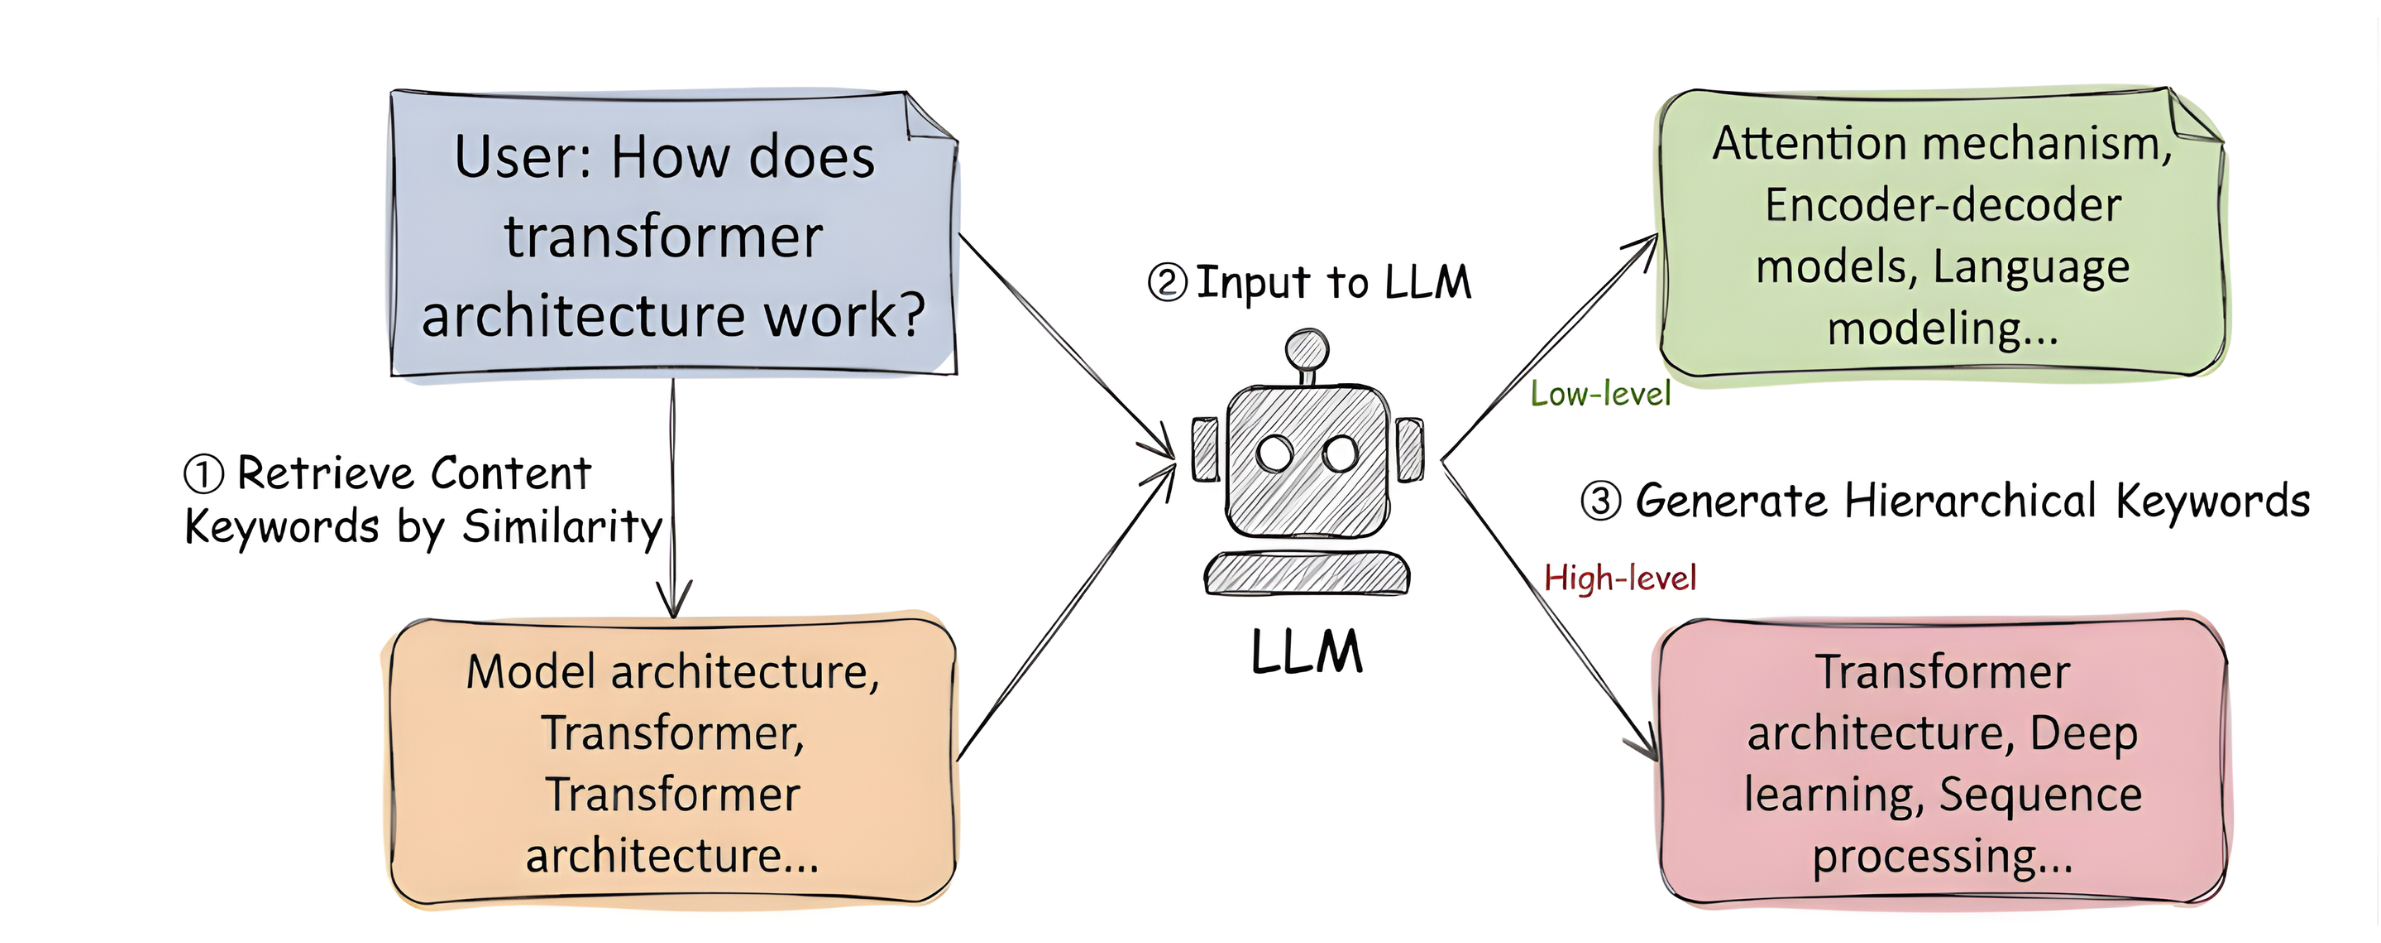
\includegraphics[width=1\textwidth]{Gambar/12.png}
            \caption{Ilustrasi Ekstraksi Kata Kunci Berdasarkan Petunjuk}
            \label{fig:Contoh Ekstraksi kata kunci}
        \end{figure}
        
        \item \textbf{Ekstraksi Informasi Lokal Berbasis Subgraf}
        
        \hspace*{0.75cm}Pada tahap ini, sistem memanfaatkan kata kunci detail ($\mathcal{K}_l$) untuk melakukan penelusuran mendalam pada graf pengetahuan. Sistem mengidentifikasi titik-titik (\textit{nodes}) yang paling relevan dan mengekstraksi informasi dari lingkungan terdekatnya untuk membentuk sebuah \textbf{subgraf} yang merepresentasikan konteks lokal. Proses ini terdiri dari beberapa langkah berikut:
        
        \begin{enumerate}[label=\textbf{\roman*.}, leftmargin=*, itemsep=3pt]
            \item \textbf{\textit{Node Matching}}: Mencocokkan node dalam graf dengan $\mathcal{K}_l$ menggunakan metrik kemiripan vektor untuk menemukan titik yang paling relevan.
            \item \textbf{\textit{Subgraph Construction}}: Membangun subgraf dengan menelusuri jalur terpendek (\textit{shortest paths}) antar node yang cocok guna mempertahankan koherensi konteks.
            \item \textbf{\textit{Pruning}}: Menyaring edge yang tidak relevan secara semantik dan menghapus node yang terisolasi untuk memastikan subgraf tetap informatif dan terfokus.
            \item \textbf{\textit{Text Unit Extraction}}: Mengambil dan meringkas unit teks (\textit{chunks}) yang paling sering muncul atau memiliki kontribusi terbesar dalam subgraf.
            \item \textbf{\textit{Edge Expansion}}: Memperluas subgraf ke tetangga satu-hop untuk menangkap konteks tambahan yang mungkin tidak terjangkau pada tahap awal.
            \item \textbf{\textit{Data Truncation}}: Memangkas jumlah node, edge, dan unit teks agar tetap berada dalam batas kapasitas memori model bahasa (\textit{token count}).
        \end{enumerate}
        
        \noindent
        Keluaran dari proses ini, yaitu $\mathcal{L}_{\text{local}}$, merepresentasikan informasi mendalam mengenai entitas yang ditanyakan oleh pengguna. Secara formal, proses ekstraksi informasi lokal dapat dituliskan sebagai:
        
        \begin{equation}
            \mathcal{L}_{\text{local}}
            = (\mathcal{E}_{\text{local}}, \mathcal{R}_{\text{local}}, \mathcal{T}_{\text{local}})
            = \text{pipeline}_{\text{local}}(\mathcal{K}_l, G).
        \end{equation}

        \begin{figure}[htbp]
            \centering
            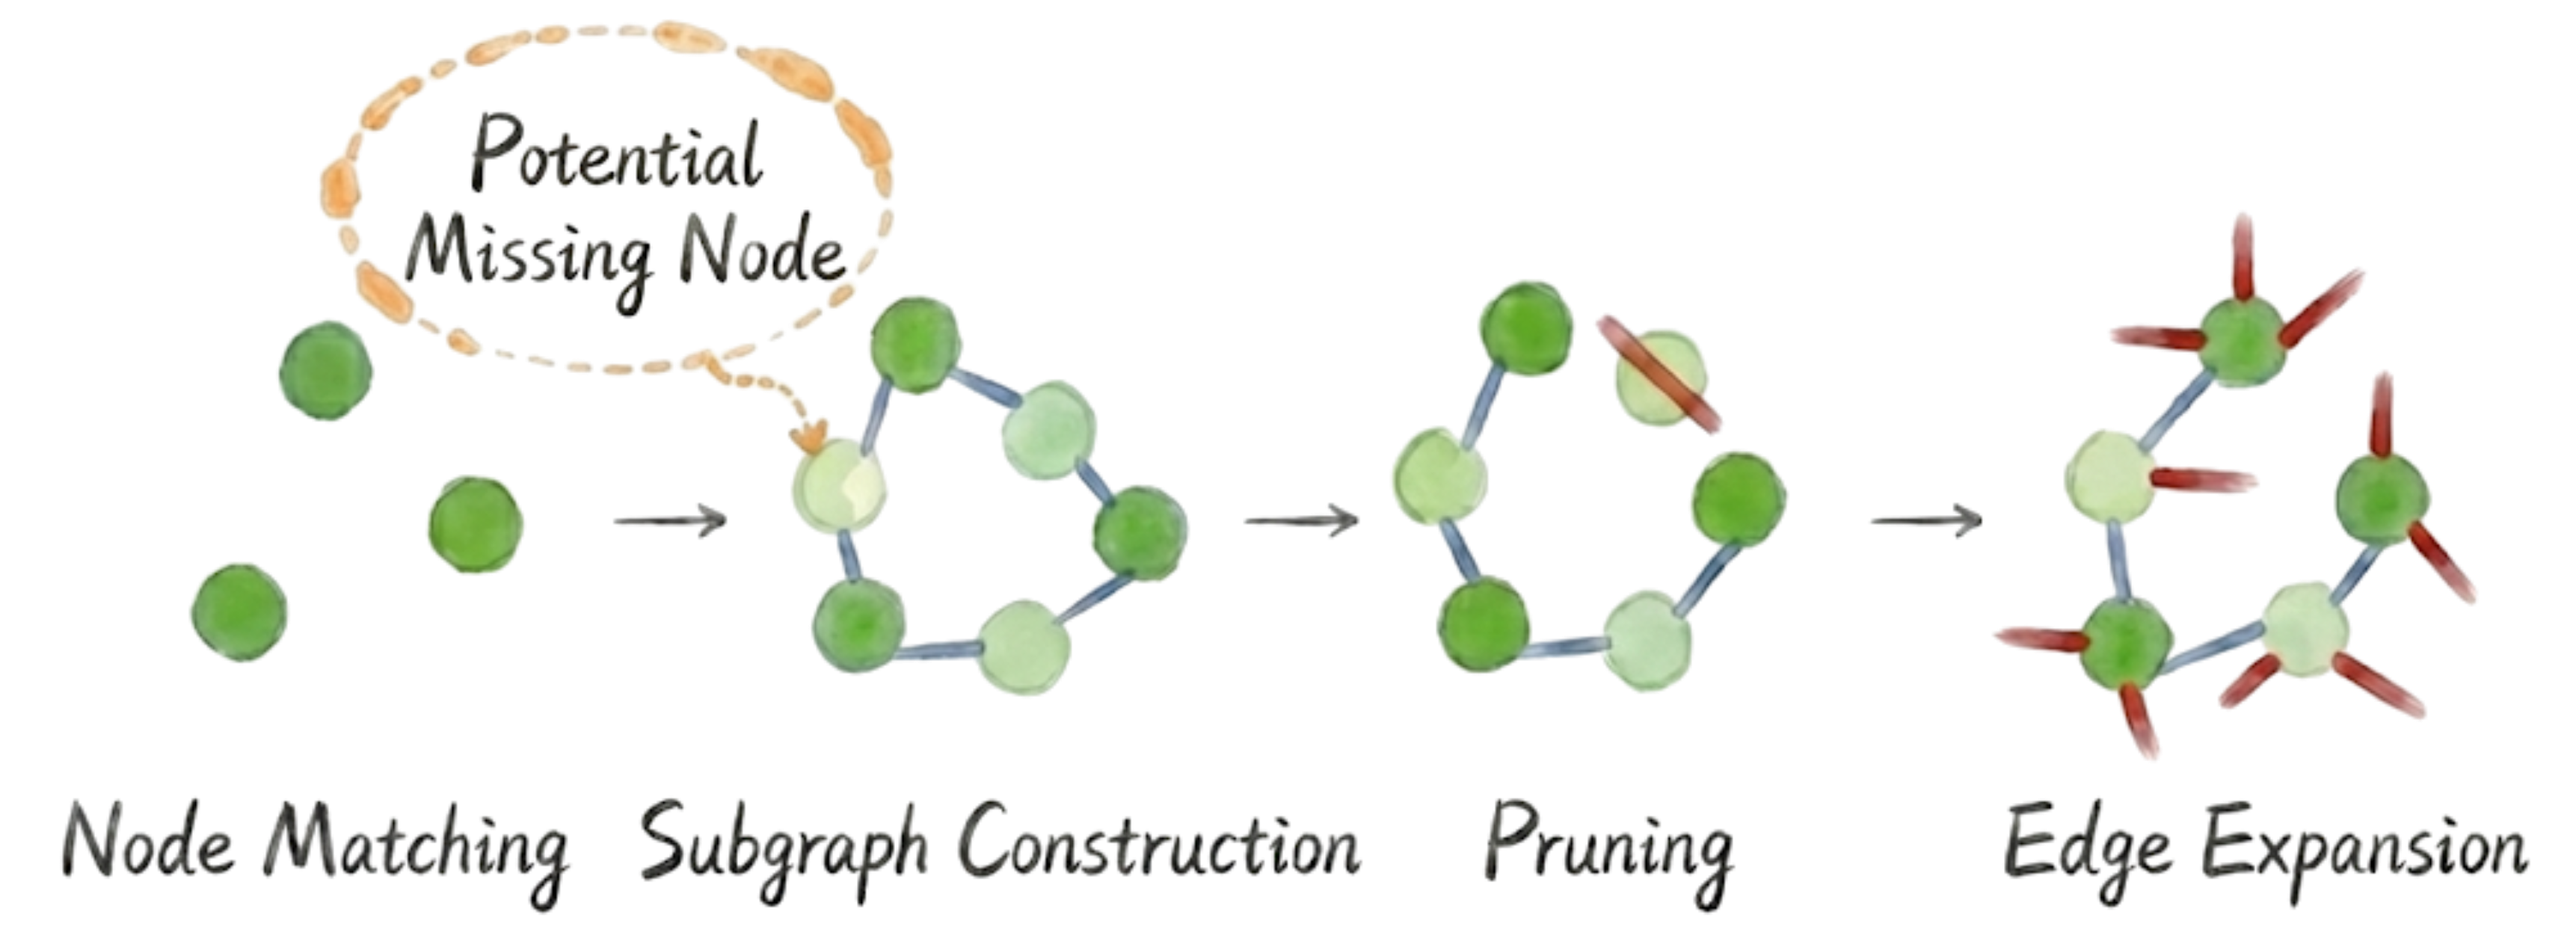
\includegraphics[width=1\textwidth]{Gambar/13.png}
            \caption{Tahapan Pembentukan Subgraf}
            \label{fig:pembentukan subgraf}
        \end{figure}
        
        \item \textbf{Ekstraksi Informasi Global}
        
        \hspace*{0.75cm}Selain menelusuri detail lokal, sistem juga membangun pemahaman tingkat tinggi dengan memanfaatkan kata kunci bertema global ($\mathcal{K}_h$). Proses ini bertujuan mengekstraksi struktur pengetahuan makro dari graf $G$ melalui tahapan sistematis berikut:
        
        \begin{enumerate}[label=\textbf{\roman*.}, leftmargin=*, itemsep=3pt]
            \item \textit{Edge retrieval}: Mengidentifikasi edge dalam basis vektor yang memiliki keselarasan tertinggi dengan $\mathcal{K}_h$.
            \item \textit{Node retrieval}: Mengambil node-node yang terhubung dengan edge terpilih.
            \item \textit{Edge data processing}: Menganalisis metadata setiap relasi untuk menghitung bobot semantik dan kekuatan keterhubungan.
            \item \textit{Integration \& ranking}: Mengintegrasikan seluruh relasi yang diperoleh dan melakukan pemeringkatan menggunakan metrik komposit (relevansi kata kunci + bobot koneksi).
            \item \textit{Text unit extraction}: Mengambil unit teks (\textit{chunks}) yang berkaitan dengan edge terpilih berdasarkan tingkat kemiripan terhadap $\mathcal{K}_h$.
            \item \textit{Data truncation}: Memangkas jumlah node, edge, dan unit teks agar tetap berada dalam batas kapasitas memori model bahasa (\textit{token count}).
        \end{enumerate}
        
        \noindent
        Tahapan ini menghasilkan keluaran berupa entitas yang saling terhubung beserta bukti teks pendukung, sehingga memungkinkan sistem memberikan jawaban yang lebih holistik. Secara formal, alur ekstraksi informasi global dapat dituliskan sebagai:
        
        \begin{equation}
            \mathcal{L}_{\text{global}} 
            = (\mathcal{E}_{\text{global}}, \mathcal{R}_{\text{global}}, \mathcal{T}_{\text{global}})
            = \text{pipeline}_{\text{global}}(\mathcal{K}_h, G).
        \end{equation}

        \item \textbf{Graph-Enhanced Generation}
        
        \hspace*{0.75cm}Tahap ini merupakan fase akhir di mana sistem menyusun jawaban berdasarkan informasi yang telah diekstraksi. Sistem menggabungkan hasil dari Subgraf Lokal dan Jaringan Relasi Global untuk membentuk kerangka konteks yang komprehensif. Integrasi ini menyatukan entitas, hubungan, serta potongan teks yang relevan sehingga menghasilkan representasi konteks yang kaya dan terstruktur. Seluruh informasi terintegrasi tersebut kemudian dimasukkan ke dalam \textit{prompt} khusus dan diproses oleh LLM untuk menghasilkan jawaban akhir yang akurat dan kontekstual.
    \end{enumerate}

    % 5. System Evaluation
    \item \textbf{System Evaluation}

    \hspace*{0.75cm}Evaluasi sistem dilakukan untuk mengukur kinerja \textit{Academic Graph-RAG} secara menyeluruh, mencakup kemampuan penelusuran (\textit{retrieval}) dan kualitas pembangkitan jawaban (\textit{generation}). Penilaian ini menggunakan metrik \textit{Context Precision} dan \textit{Context Recall} untuk memastikan relevansi konteks yang diambil dari \textit{Knowledge Graph} dan basis data vektor, serta metrik \textit{Faithfulness}, \textit{Answer Relevance}, dan \textit{Traceability} untuk menjamin akurasi dan transparansi jawaban yang dihasilkan LLM. Sistem yang efektif ditandai dengan tingginya nilai presisi dan kelengkapan konteks, serta jawaban yang konsisten dengan sumber (\textit{faithful}), relevan dengan kueri pengguna, dan memiliki sitasi yang dapat dilacak ke dokumen asli.

    % 6. GUI Implementation
    \item \textbf{GUI Implementation}

    \hspace*{0.75cm}Desain antarmuka pengguna (\textit{Graphical User Interface}) berbasis Streamlit dikembangkan secara modular untuk mendukung proses penemuan pengetahuan akademik. Pada aplikasi Asisten Tinjauan Literatur, antarmuka ini terdiri atas beberapa halaman interaktif yang memungkinkan pengguna memasukkan kueri pencarian, menjelajahi visualisasi \textit{Knowledge Graph}, serta memperoleh sintesis jawaban dari dokumen ilmiah secara \textit{real-time}.

\end{enumerate}

\section{JADWAL PENELITIAN}

Kegiatan penelitian ini akan mengikuti jadwal yang telah disusun pada ~\ref{tab:jadwal-penelitian}. Jadwal dirancang untuk mencakup seluruh tahapan penelitian dari persiapan hingga penyelesaian thesis. Untuk setiap kegiatan diblok dengan sesuai dengan minggu dan bulan yang ada. Jadwal fleksibel dan dapat disesuaikan berdasarkan perkembangan penelitian dan ketersediaan resources.

\begin{table}[htbp]
    \centering
    \caption{Pelaksanaan Penelitian}
    \label{tab:jadwal-penelitian}
    \renewcommand{\arraystretch}{1.3} 
    \small 
    \begin{tabular}{|p{3.5cm}|c|c|c|c|c|c|c|c|c|c|c|c|}
        \hline
        \multirow{2}{*}{\textbf{Kegiatan}} & \multicolumn{4}{c|}{\textbf{Bulan I}} & \multicolumn{4}{c|}{\textbf{Bulan II}} & \multicolumn{4}{c|}{\textbf{Bulan III}} \\
        \cline{2-13}
        & 1 & 2 & 3 & 4 & 1 & 2 & 3 & 4 & 1 & 2 & 3 & 4 \\
        \hline
        Studi Literatur & \cellcolor{gray!40} & \cellcolor{gray!40} & & & & & & & & & & \\
        \hline
        Pengambilan Data & & & \cellcolor{gray!40} & \cellcolor{gray!40} & \cellcolor{gray!40} & & & & & & & \\
        \hline
        Pengolahan Data & & & & & \cellcolor{gray!40} & \cellcolor{gray!40} & \cellcolor{gray!40} & & & & & \\
        \hline
        KG Construction & & & & & & \cellcolor{gray!40} & \cellcolor{gray!40} & \cellcolor{gray!40} & \cellcolor{gray!40} & & & \\
        \hline
        Implementasi Hybrid RAG & & & & & & & & \cellcolor{gray!40} & \cellcolor{gray!40} & \cellcolor{gray!40} & & \\
        \hline
        Evaluasi & & & & & & & & & & \cellcolor{gray!40} & \cellcolor{gray!40} & \\
        \hline
        
        Penulisan Skripsi & & & & & \cellcolor{gray!40} & \cellcolor{gray!40} & \cellcolor{gray!40} & \cellcolor{gray!40} & \cellcolor{gray!40} & \cellcolor{gray!40} & \cellcolor{gray!40} & \cellcolor{gray!40} \\
        \hline
    \end{tabular}
\end{table}
